% Created 2018-04-24 Tue 00:43
% Intended LaTeX compiler: xelatex
\documentclass[a4paper,11pt]{article}
\usepackage{graphicx}
\usepackage{grffile}
\usepackage{longtable}
\usepackage{wrapfig}
\usepackage{rotating}
\usepackage[normalem]{ulem}
\usepackage{amsmath}
\usepackage{textcomp}
\usepackage{amssymb}
\usepackage{capt-of}
\usepackage{hyperref}
\usepackage{ctex}
\setCJKmainfont{SimSun}
\author{骆炜}
\date{\today}
\title{猫狗大战(最终篇)}
\hypersetup{
 pdfauthor={骆炜},
 pdftitle={猫狗大战(最终篇)},
 pdfkeywords={},
 pdfsubject={},
 pdfcreator={Emacs 25.3.1 (Org mode 9.1.8)}, 
 pdflang={English}}
\begin{document}

\maketitle
\tableofcontents


\section{项目概览}
\label{sec:org964cc8f}
本项目基于Kaggle公开训练的和测试数据集实现对图像中猫狗进行图像识别。本项目涵盖数据处理,模型选择和搭建以及最终测试等主要步骤。
\section{数据研究}
\label{sec:org8f0ac97}
本项目有Kaggle提供了25000张训练照片和12500测试照片。对于数据的研究主要针对训练照片展开,而测试照片将会原封不动保留到测试步骤。
\subsection{预理筛除}
\label{sec:orgadcee09}
首先,根据这篇\href{https://github.com/ypwhs/dogs\_vs\_cats}{Github内容}\footnote{\url{https://github.com/ypwhs/dogs\_vs\_cats}}所述的方法创建符号链接,避免复制一遍照片。其次,依据\href{https://zhuanlan.zhihu.com/p/34068451}{这篇博客}\footnote{\url{https://zhuanlan.zhihu.com/p/34068451}}所提示的信息,我也对Kaggle的数据集进行了筛查。所用的方法和博客作者类似,通过已经在ImageNet数据集下进行了训练,对包括猫狗在内的多个类别能进行有效的判断。在 \textbf{pre\_check\_img.py} 中有代码的具体实现。结合时下比较精确的三个的网络模型,ResNet50,Xception和Inception-RestnetV2,共同对原数据集进行预筛查。每个模型最终的结果选择TOP-10作为依据,即如果前10个判断中有出现猫/狗相关的判断,即可认为这张图片中存在猫/狗,反之则需要添加到排除列表中。  

\subsection{数据增强}
\label{sec:orgd93702f}
数据增强是一系列扩充图像数据的方法,通过裁切、添加噪音、改变颜色等手段,对原始照片进行处理,进而生成更多的用以训练的数据,弥补数据量不足造成的过拟合问题。本项目使用Github中开源项目Imgaug\footnote{\url{https://github.com/aleju/imgaug}}进行数据增强的图片生成。Imgaug集成了多种数据增强手段,可以方便的调用。本项目选用了四种手段进行预处理,每张照片选择两个处理手法,即一张照片可以生成六张照片。示例如图\ref{fig:cats}所示。通过两个python文件 \textbf{create\_aug\_fotos.py} 和 \textbf{data\_aug\_tool.py} 可以将筛选后的原始训练文件生成约15万张猫狗照片进行训练。

\begin{figure}[htb]
\centering
\subfigure{
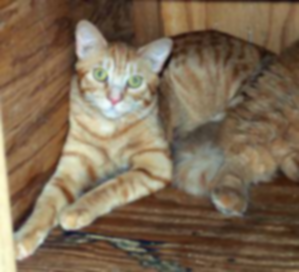
\includegraphics[scale=0.4]{./figure/cat1.jpg}
\label{fig:cat1}
}
\subfigure{
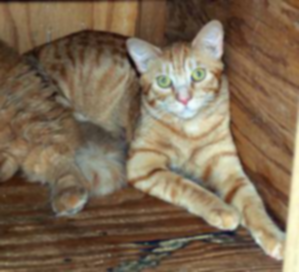
\includegraphics[scale=0.4]{./figure/cat2.jpg}
\label{fig:cat2}
}
\subfigure{
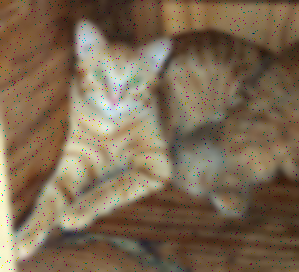
\includegraphics[scale=0.4]{./figure/cat3.jpg}
\label{fig:cat3}
}
\subfigure{
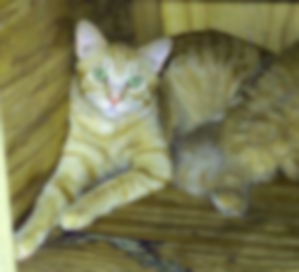
\includegraphics[scale=0.4]{./figure/cat4.jpg}
\label{fig:cat4}
}
\subfigure{
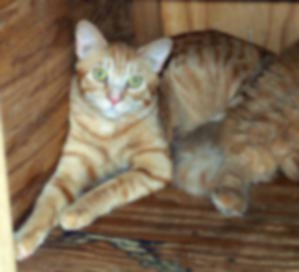
\includegraphics[scale=0.4]{./figure/cat5.jpg}
\label{fig:cat5}
}
\subfigure{
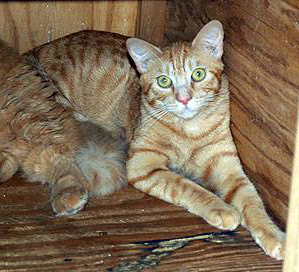
\includegraphics[scale=0.4]{./figure/cat6.jpg}
\label{fig:cat6}
}
\caption{Imgaug处理结果}
\label{fig:cats}
\end{figure}

\section{算法与方法}
\label{sec:org22eece6}
由于Keras提供了非常便捷的功能,大部分算法部分的结构不需要我们自己重新处理。为了提高最终的识别精度,本项目结合了之前预筛选所选用的三种模型进行迁移学习,最后加入自定义的层进行训练。
\section{测试结果}
\label{sec:org5109912}
\subsection{生成特征向量}
\label{sec:orgd4af9e4}
使用特征向量和训练数据生成特征向量,有利于快速进行训练。使用原始训练数据得到的特征向量.h5文件大约300多MB,而使用数据增强方式生成的照片每个.h5文件大约1.5GB。具体代码详见python或是jupyter notebook文件。
\subsection{测试结果}
\label{sec:org67d22bb}
在测试的时候,将预生成好的.h5文件载入,连接上自定义的网络层进行训练,并将结果以Kaggle要求的csv文件方式保存。最后将生成的csv文件上传至Kaggle平台,得到如下测试结果,图\ref{fig:kaggle}。

\begin{figure}[htb]
\centering
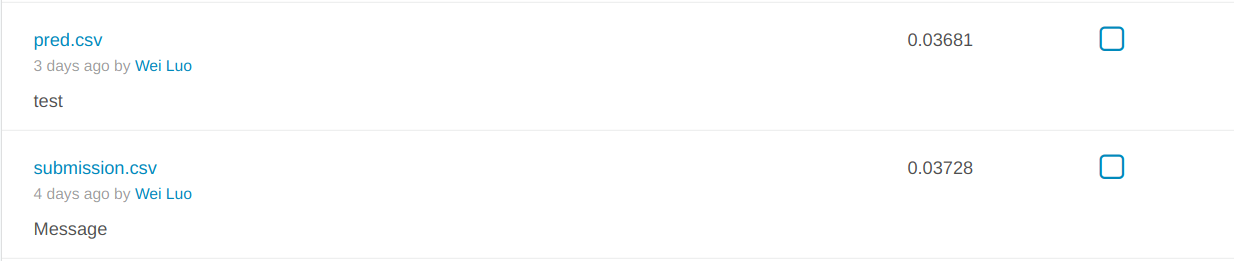
\includegraphics[scale=0.25]{./figure/record.png}
\caption{Kaggle测试结果}
\label{fig:kaggle}
\end{figure}

最终结果为,以数据增强后训练的模型比直接使用原训练数据的模型有较好的测试结果(0.03681 vs 0.03728)。之后结合模型结构优化,可能会取得更好的结果,因为增强后数据的量更适合训练复杂的模型。
\section{项目附件及其说明}
\label{sec:org63942ee}

现在对Github提交的文件进行补充说明: 
\begin{enumerate}
\item final\_paper.pdf -- 最终报告文稿
\item create\_symbol\_link/\_2.py -- 生成图像的符号链接
\item pre\_check\_img.py, remove\_list\_cat/dog.txt -- 判断是否非猫非狗
\item create\_aug\_fotos.py data\_aug\_tool.py  -- 数据增强工具
\item Feature\_Gen.py  -- 生成特征向量
\item TrainingandTesting.py -- 训练并获得结果
\item submission\_first/final.csv  -- kaggle提交文件
\item Final\_jupyter\_notebook.ipynb  -- 解释性jupyter notebook
\end{enumerate}
\end{document}